\chapter[Research Methodology]{Research Methodology}

\section{Background}

As I stated in Chapter 1, we are interested in analyzing both the quantitative effects of the \gls{cita} system on student grades as well as student perceptions of the system. Thus, we will use a mixed method study in order to gain a complete understanding of \gls{cita} on \gls{chip}. Quantitative analysis will be used to find trends in student grades between classes that do and do not use the program. The research team will conduct a parallel qualitative study to determine student reactions to the program and how they feel their learning was affected. A breakdown of our methodology is shown in Figure \ref{fig:analysisFlowchart}.

\begin{figure}[h]
	\centering
	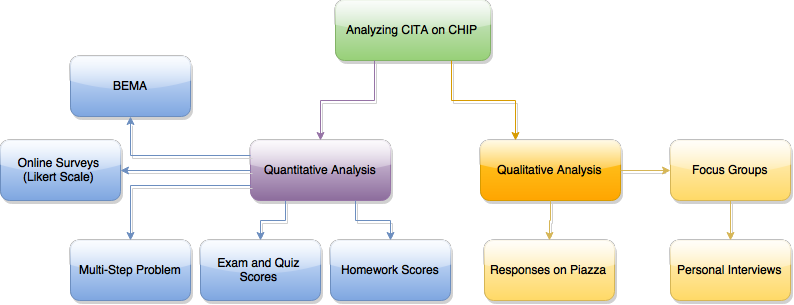
\includegraphics[width=6in]{img/chapter3/analysis_flowchart}
	\caption[Flowchart of Analysis Techniques]{Flowchart of Analysis Techniques}
  \label{fig:analysisFlowchart}
\end{figure}

\section{Quantitative Analysis}

\subsection{Homework Scores}

Since the \gls{cita} on \gls{chip} program is centered around homework assignments, the research team needs to analyze how students perform on their weekly homework problems with and without \gls{cita}. This involves not only looking at scores as a whole, but also diving into each problem individually, checking to see what paths students took to solve each problem. Our control groups for the homework assignments will be the summer 2014, fall 2014, and spring 2015 semesters; these classes will be compared to summer 2015, fall 2015, spring 2016, and summer 2016 semesters. Thus, we will get a good sense of how students perform with and without scaffolding provided by \gls{cita}.

The research team can track the level to which students delve into the tutorial using the statistical analysis tools on \gls{chip}. Thus, the research team can determine who specifically is using \gls{cita}, how diligently they are using the hints, and how they traverse through the problem. Throughout this study, I will analyze:

\begin{enumerate}
\item How deep students get into the \gls{cita} structure before entering an answer.
\item How many attempts students use before, during, and after accessing the \gls{cita} tutorial.
\item Whether or not students obtain a correct answer using the \gls{cita} system.
\item After using \gls{cita} on one problem is it used on every problem
\item How homework scores relate to \gls{bema} scores, quiz scores, and exam scores.
\end{enumerate}

\subsection{Quiz and Exam Scores}

Homework scores are useful to judge whether students can complete assignments with a tutorial, but they do not tell us how students do when the tutorial is removed. We need to look at quiz and exam data for each class in order to determine if the scaffolding provided by \gls{cita} improved student problem solving and conceptual understanding. Our control groups for the quizzes and exams will be the summer 2014, fall 2014, and spring 2015 semesters; these classes will be compared to summer 2015, fall 2015, spring 2016, and summer 2016 semesters. Throughout this study, I will analyze:

\begin{enumerate}
\item When during the semester did students start using \gls{cita} and how this correlates with quiz and exam scores.
\item Comparison of performance on simple one-step problems vs. more complicated multi-step problems.
\item Student improvement between the first and second exams as well as the final exam.
\end{enumerate}

\subsection{Brief Electricity and Magnetism Assessment (BEMA)}

Concept inventories and assessment instruments are a useful method of assessing student knowledge of the material; however, they are not simply tests that can be quickly put together and administered year after year. Lindell and Ding describe how it takes years to determine the validity and reliability of the results of a given concept inventory. They describe how reliability (precision) and validity (accuracy) play a role in the inventories and cite how factors such as age, course structure, geography, language, delivery of the tests, and wording of questions can influence the results of the assessment\cite{lindell2012}.

The \gls{bema} was developed by Ruth Chabay, Bruce Sherwood, and Fred Reif in 1997. Although it was originally designed to measure student retention of electricity and magnetism concepts three months to five semesters after completing an introductory electricity and magnetism course, it is now often used to analyze student learning between the beginning and end of the semester. It is a useful tool to assess the understanding of electricity and magnetism concepts that are covered in a college-level calculus-based introductory physics course\cite{ding2006}.

The \gls{bema} is a multiple choice test consisting of qualitative questions and a few simple calculations. Lin Ding et al. performed an analysis of the \gls{bema}, showing that it is a reliable assessment tool for introductory electricity and magnetism courses\cite{ding2006}. Thus, we will use the \gls{bema} exam to assess student conceptual understanding of introductory electromagnetism topics. Our control groups for the \gls{bema} is the spring 2015 semesters; this class will be compared to summer 2015, fall 2015, spring 2016, and summer 2016 semesters.

\subsection{Multi-Step Problem}

Chabay and Sherwood demonstrated a technique to analyze how well students can solve a non-trivial multi-step problem\cite{sherwood2005, chabay2014}. They gave their students a complex problem during recitation and tracked how far students made it into the analysis before getting stuck. Then, they plotted the curves for how many students made it to certain points in the problem.

I plan to use this method to analyze how well students can solve a complex problem without the aid of a scaffold. The control group for this analysis will be the spring 2015 semester. The experimental groups will be the fall 2015 and spring 2016 semesters. See the appendix for the question text and rubric that will be used in the coming semesters.

\subsection{Online Surveys}

Capping off our quantitative analysis is a series of online surveys given to students. These surveys are not required; in fact, students can gain a small number of bonus points if they take the time to fill them out (i.e. ten points, approximately the weight of one recitation quiz). The purpose of these surveys is to collect demographic data and get a broad sense of how students felt about the \gls{cita} system. This will be used in the analysis to pick out any trends between different groups of students (i.e. domestic vs. foreign, male vs. female, etc.). See the appendices for copies of the demographics survey and the student exit survey.

\section{Qualitative Inquiry}

\subsection{Strategy of Inquiry}

We will use purposeful sampling as our design strategy. Patton defines this strategy as one where the researcher chooses specific participants for the study in order to gain insight about a specific phenomenon. He describes how cases are selected because they are ``information rich''. Purposeful sampling leads to great insight about a specific phenomenon, but it cannot be generalized to a population as a whole\cite{patton2015}. In our study, the research team will gain a lot of insight into the opinions of students using the \gls{cita} system, but these opinions will not necessarily be applicable to homework systems outside of PHYS 24100 at Purdue University.

We will use focus group sessions to gather information about student's opinions of the \gls{cita} program. One of the many strengths of focus groups is that they are flexible; they can be used for exploratory, explanatory, and evaluative research. Due to this flexibility, focus groups can naturally fit into mixed method research.

Focus groups create a large volume of data with a range of viewpoints. Furthermore, a skilled moderator can ensure that this data has limited researcher influence. In a one-on-one interview, the interviethe research teamr cannot help but insert some of his or her own views into the discussion due to the questions asked. however, a focus group can “veer off topic”. Since the group can discuss what they feel is important, they can illuminate important points that the moderator might miss.

Ideally, a focus group should recruit strangers that have knowledge of the material, but no knowledge of each other's opinions. Recruiting total strangers will be somewhat difficult in this study. We will not know if the students in my focus group session have worked together on physics homework beforehand. however, by separating the students in the same section, the research team should keep the populations reasonably homogeneous, yet randomized.

We would like to divide the pool of student volunteers up into six groups. First, I will separate them if they the research teamre in the online or on-campus sections of Electricity and Optics. Then, I will divide them up based on their overall view of the tutorials - generally positive, generally negative, or neutral. Although a student’s opinion on the interactive tutorials would not be considered “highly confrontational”, as Hennink describes, it will be useful to hold separate groups for each viewpoint so as to probe each opinion fully.

I would like to get six people for each group (a total of 36 people per semester). If the research team cannot collect enough volunteers or if the volunteers are skethe research teamd one way or another, the research team will keep the number in each group the same in order to make sure that there are good discussions. Instead, the research team will mix the neutral population with the two extremes, being careful to balance each side out.

If students are interested in sharing more information after the focus group session has ended, the research team will give them the chance to come in for a one-on-one interview. There, the research team can delve deeper into their own individual thoughts on \gls{cita}.

\subsection{The Role of the Researchers}

In qualitative studeies the researcher must acknowledge that his or her presence in the experiment can alter the ansthe research teamrs given by the participants. Thus, researchers must take time beforehand to determine how their presence might skew the data as the research teamll as how to minimize this artifact\cite{denzin2012}. In this study the principle investigators are myself (Cyrus Vandrevala), Dr. Lynn Bryan, Dr. Andrew Hirsch, Dr. Hisao Nakanishi, and Dr. Laura Pyrak-Nolte. The core team will receive advice and guidance from a variety of sources including teaching assistants in PHYS 24100 and members of the physics education research group at Purdue University.

I have been a teaching assistant for PHYS 24100 and PHYS 24100D since the fall semester in 2011. Additionally, I have coordinated the course during summer sessions and helped develop the online sections. This includes editing course videos and setting up the online forum\cite{piazza}. I am currently a senior teaching assistant at Purdue, providing advice to other graduate students who are teaching Electricity and Optics. Throughout this study my teaching duties are going to mainly be managing the online forum. Thus, I will not be grading any student assignments or assigning any final grades. This will hopefully make students feel more at ease when I conduct focus group sessions and interviews. I will try to recruit one or two PHYS 24100 teaching assistants to help me record the interviews.

Dr. Hisao Nakanishi is the ``father'' of \gls{chip} at Purdue University. He is one of the primary developers of the system; to this day he continually makes updates to its content, functionality, and robustness. Due to his experience with \gls{chip}, Dr. Nakanishi develops and implements most of the new structures that the research team are building in this project. He also addresses student questions sent through \gls{chip} about possible errors in the codebase. On some rare occasions, he does ansthe research teamr questions about PHYS 24100 and PHYS 24100D assignments as the research teamll. Since Dr. Nakanishi is not directly tied to PHYS 24100 or PHYS 24100D, he could potentially aid with focus group sessions or student interviews if I cannot find graduate student volunteers.

Dr. Laura Pyrak-Nolte has taught PHYS 24100 and PHYS 24100D since 2005 and coordinated the course since the fall 2011 semester. As the course coordinator, Dr. Pyrak-Nolte is in charge of creating the curriculum for the class, designing midterm and final exams, assigning final grades, and approving all new changes to the homework system that the research team are developing. Additionally, she is the lecturer that is seen and heard in the online lecture videos shown to the PHYS 24100D class. Due to the fact that Dr. Laura Pyrak-Nolte is the coordinator for the class, she should not conduct any of the focus group sessions or interviews with the students. There might be a conflict of interest.

Drs. Lynn Bryan and Andrew Hirsch are the research teamll versed in educational theory, providing a solid check of the pedagogy in this project. Dr. Hirsch is the interim head of the physics department at Purdue University and Dr. Bryan has a dual appointment within physics and education. Neither of them are directly involved with PHYS 24100 or PHYS 24100D, so they can potentially help with focus groups or interviews should the need arise.

\subsection{Planned Analysis Procedures}

Once the research team have the transcripts and recordings from focus group sessions and followup personal interviews, the research team will carefully parse the data to find patterns. First, the research team will transcribe any recordings so that they are easier to analyze. Then, the research team will sift through them, looking for key words and phrases that describe how students view the program. Finally, the research team will synthesize these building blocks into a theory of how introductory physics students at Purdue University view the \gls{cita} program. We will use inductive analysis and creative synthesis as the analysis strategy.

\section{Data Collection Procedures}

It is important to protect student records when doing a study like this. \gls{chip} already uses strong security to protect student records - all students and instructors need to sign into the system using a unique username and password. Additionally, the support staff at Purdue University makes sure that students and instructors are only given permission to access data that is pertinent to them.

We will take additional measures to ensure that all of the data from interviews and focus groups are protected. Whenever the research team transcribe data, the research team will identify participants with letters or numbers rather than names (participant A, B, C, etc.). If the research team do decide to store this data on \gls{chip}, it will be put in a separate, private classroom that only the researchers will be able to access.

Finally, the research team will only analyze grade data after the semester has ended. This will ensure no conflict of interest between the study and student grades. Interviews might have to take place during the semester due to scheduling. however, as stated above the participants will be anonymized in order to protect their identity.




\section{Setting and Context}

The population that the research team are studying is engineering and science students at Purdue University who are taking their second semester of introductory physics. This population contains both domestic and foreign students.

Most of them take this course to get to engineering classes.

The combined yearly enrollment of PHYS 24100 and PHYS 24100D has an average of about 1500 students from science and engineering. Additionally, the research team have seen an increase in the number of students in online sections ever since the distance learning course was started in the summer semester of 2012.

\section{Timeline and Budget}

The timeline for the development, implementation, and assessment of \gls{cita} on \gls{chip} is shown in Table \ref{tab:timeline}. As of the end of the summer semester in 2015, the project is on schedule.

\pagebreak

\begin{landscape}
\begin{table}[!ht]
  \centering
  \begin{tabular}{|l|l|l|}
    \hline
    \textbf{Semester} & \textbf{CITA Content} & \textbf{Learning Assessment}\\
	\hline
	Spring 2015 & Create Branching Help Button for \gls{chip} & \\
	& Create \gls{cita} Homework Problems & \\
	& Design \gls{gui} for \gls{chip} & \\
	\hline
	Summer 2015 & Create \gls{cita} Homework Problems & Begin Preliminary Work on Muffin\\
	& Beta Test of \gls{cita} Homework Problems &  \\
	\hline
	Fall 2015 & Update \gls{gui} for \gls{chip} & Analyze \gls{cita} Data from Spring 2015 \\
	& Update Assessment Tools on \gls{chip} & Analyze \gls{cita} Data from Summer 2015 \\
	& Expand \gls{cita} Problems & Finalize Muffin \\
	\hline
	Spring 2016 & Expand \gls{cita} Problems & Analyze \gls{cita} Data from Fall 2015 \\
	& Create Interactive Graphics for \gls{cita} & Analyze Class Data from 2012-2014 \\
	\hline
	Summer 2016 & Expand \gls{cita} Problems & Analyze \gls{cita} Data from Spring 2016 \\
	& Expand Interactive Graphics for \gls{cita} & \\
	\hline
	Fall 2016 & Expand \gls{cita} Problems & Analyze \gls{cita} Data from Summer 2016 \\
	& Expand Interactive Graphics for \gls{cita} & \\
	\hline
  \end{tabular}
  \caption{Project Timeline}
  \label{tab:timeline}
\end{table}
\end{landscape}

\pagebreak

This work is funded by a grant through the College of Science at Purdue University. The first part of the grant will last through the year 2015. Then, the grant can be renethe research teamd for another year (2016).